\documentclass{article}
\usepackage{graphicx} % Required for inserting images
\usepackage{float}
\usepackage{parskip}
\usepackage{hyperref}
\usepackage{apacite}
\usepackage{enumitem} % For nested lists in maze generation section
\usepackage[margin=1.5in]{geometry} % Reduce horizontal padding

\title{Simple Doom Game Clone in Three.js}
\author{Elias Nijs \& René Van Der Schueren}
\date{May 2025}

% Custom title page information
\newcommand{\courseinfo}{Computer Graphics (E016712A)}
\newcommand{\academicyear}{Academic Year 2024/2025}
\newcommand{\university}{GHENT UNIVERSITY}

\begin{document}

% Custom title page
\begin{titlepage}
    \centering
    \vspace*{1cm}
    
    \Huge
    \textbf{Simple Doom Game Clone in Three.js}\\
    \vspace{1.5cm}
    
    \Large
    \textbf{\courseinfo}\\
    \vspace{0.5cm}
    
    \large
    \university\\
    \vspace{0.5cm}
    
    \vspace{1.5cm}
    
    \Large
    Elias Nijs \& René Van Der Schueren\\
    \vspace{0.5cm}
    
    \large
    \academicyear\\
    \vspace{0.5cm}
    
    \large
    May 2025\\
    
\end{titlepage}

\pagebreak

\tableofcontents

\pagebreak

\begin{figure}[H]
    \centering
    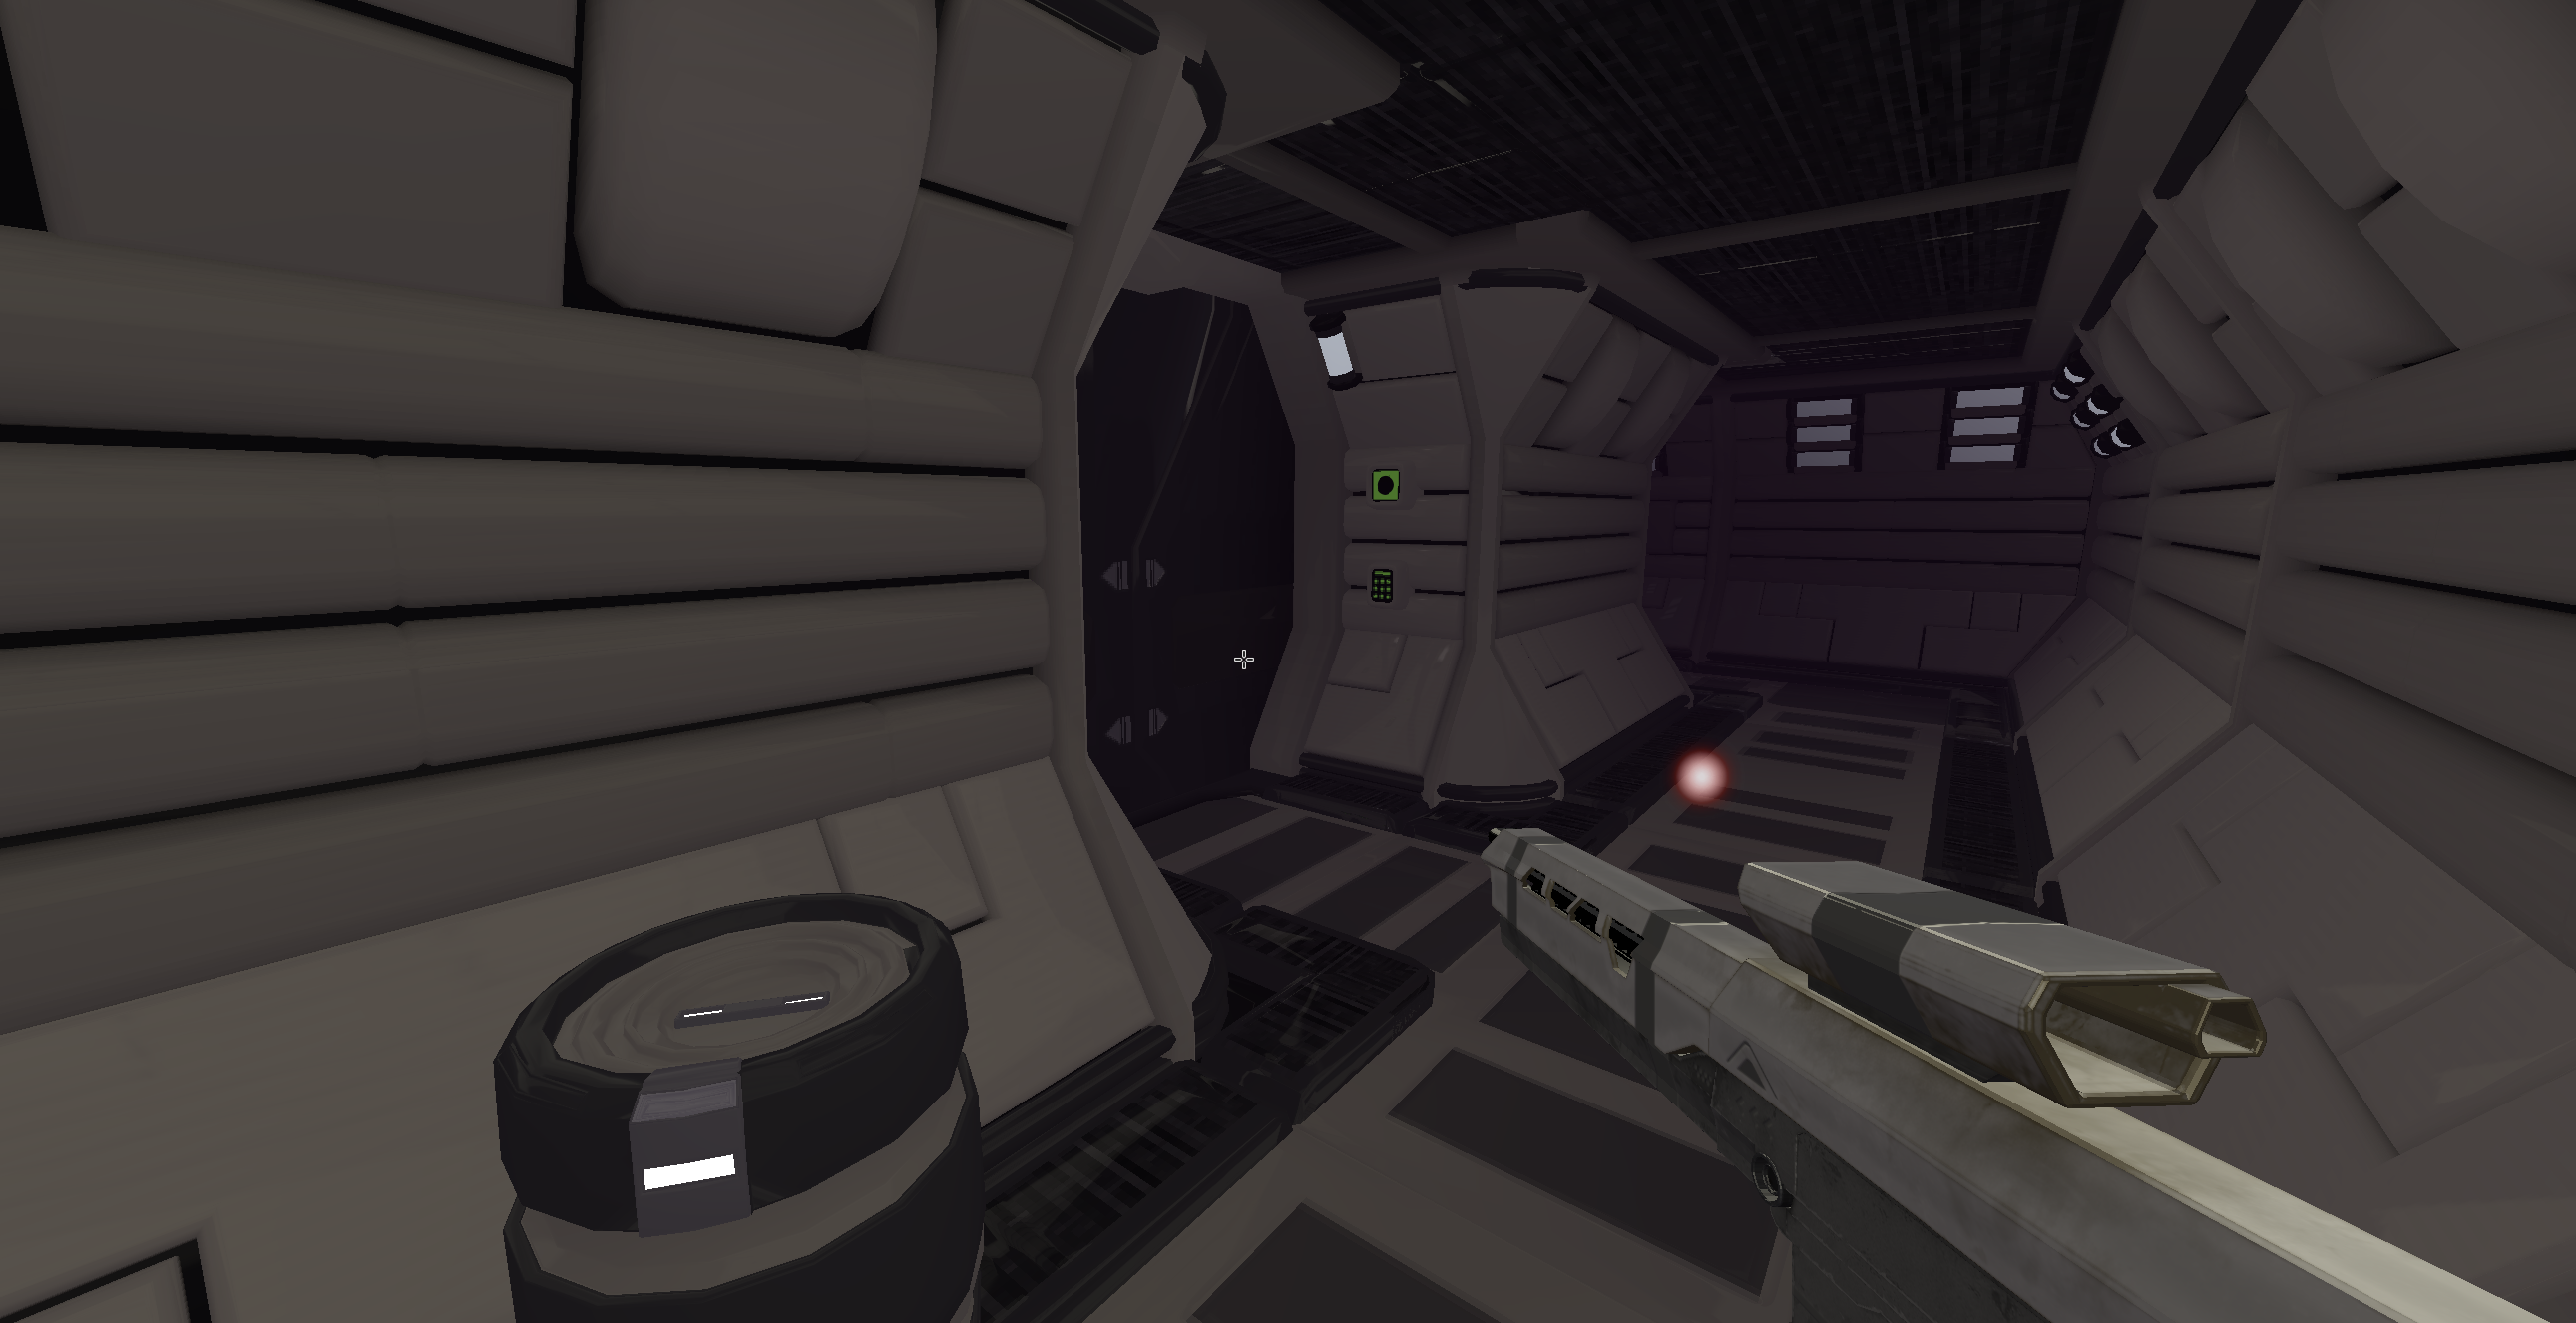
\includegraphics[width=\textwidth]{diagrams/gameplay.png}
    \caption{Gameplay screenshot of our Doom-inspired game implemented in Three.js.}
    \label{fig:gameplay-main}
\end{figure}

\section{Introduction}\label{sec:introduction}
\subsection{Tech Choices}
Our project leverages Three.js, a lightweight, cross-browser JavaScript library that abstracts WebGL, making 3D graphics programming significantly more accessible. It provides a comprehensive set of features for creating and displaying animated 3D computer graphics in web browsers without requiring users to install additional plugins. Three.js was the best option for its robust ecosystem, extensive documentation, and optimized performance for web-based 3D rendering.

Our development workflow is built around Vite, a modern frontend build tool that provides an extremely fast development server through native ES modules.

We implemented the entire codebase in TypeScript rather than vanilla JavaScript to enhance our development process. TypeScript's static typing helps catch errors during development rather than at runtime, significantly improving code reliability. The explicit type definitions serve as built-in documentation, making it easier for team members to understand each other's code and collaborate effectively.

\subsection{Gameplay Overview}
Our game is a first-person shooter inspired by the classic Doom, implemented using Three.js. Players navigate through procedurally generated mazes, interact with doors, follow path markers, and encounter various props while trying to reach their destination. Players can also shoot their gun to open doors, adding a combat element to the navigation mechanics.

\begin{figure}[H]
    \centering
    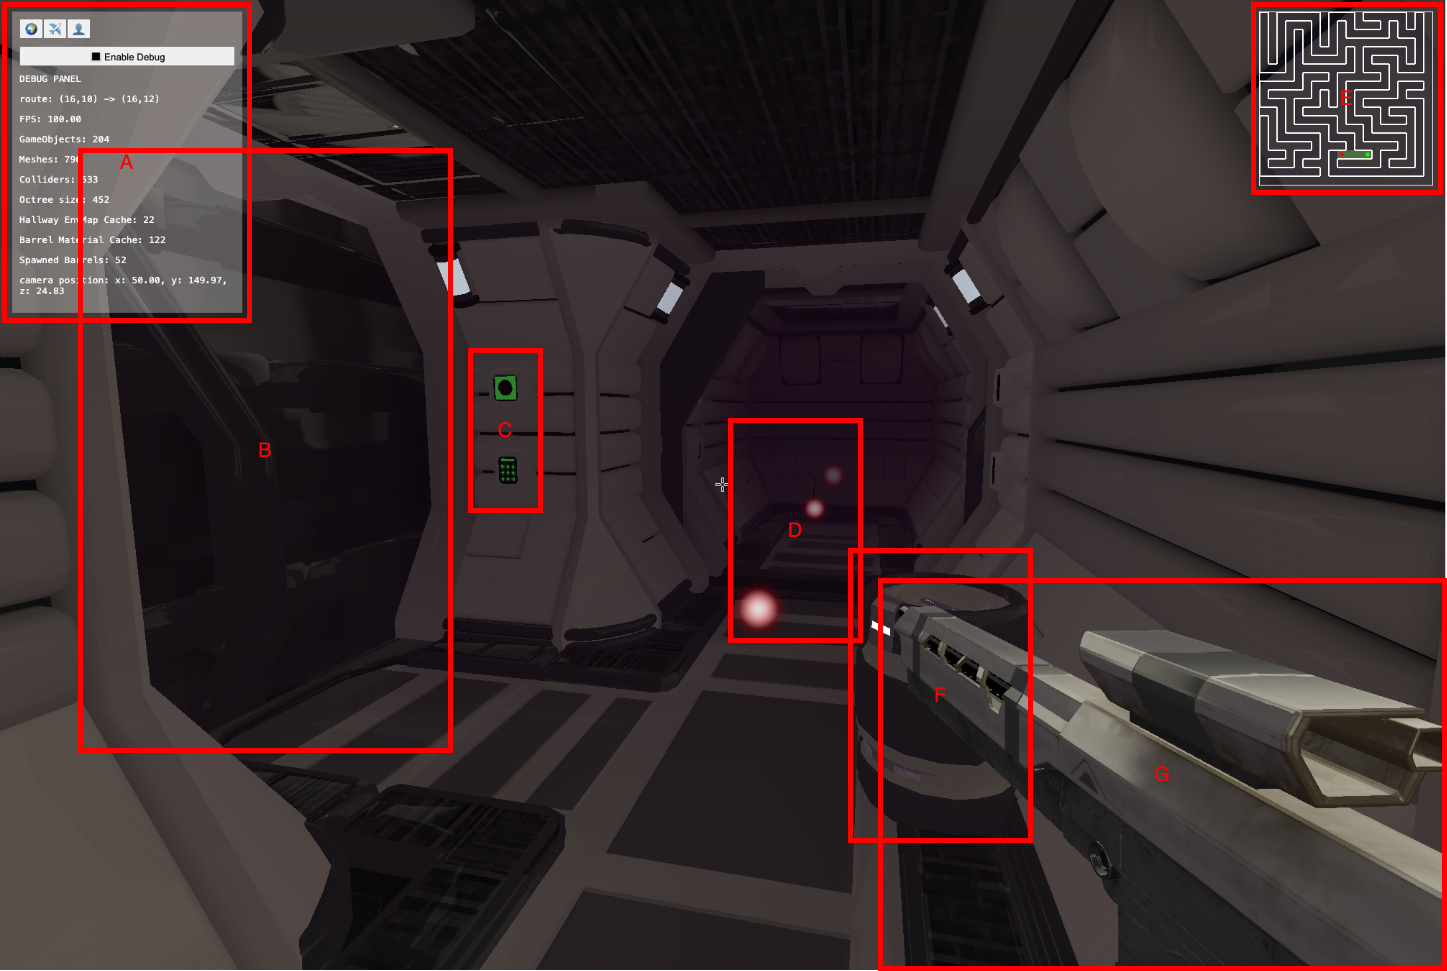
\includegraphics[width=\textwidth]{diagrams/screenshot.png}
    \caption{Gameplay screenshot showing key elements: (A) Debug menu for adjusting game parameters, (B) Closed door with its control panel (C), (D) Path markers guiding the player through an open door, (E) Mini-map displaying player position and path to destination, (F) Barrel spawned as a random prop, and (G) Weapon in gun mode.}
    \label{fig:gameplay-overview}
\end{figure}

Figure \ref{fig:gameplay-overview} illustrates the main gameplay elements:
\begin{itemize}
    \item \textbf{A:} Debug menu that allows changing camera settings, enabling debug mode, and displays game engine statistics.
    \item \textbf{B:} A door that was previously opened, allowing passage through the maze.
    \item \textbf{C:} Door control panel that can be activated by shooting it with the player's weapon.
    \item \textbf{D:} Path markers showing the optimal route to the destination, guiding the player through an open door.
    \item \textbf{E:} Mini-map displaying the player's current position and the path to the destination.
    \item \textbf{F:} Barrel that was procedurally spawned as a random prop in the environment.
    \item \textbf{G:} The player's weapon in gun mode.
\end{itemize}


\section{Maze Generation}
First, we will start by explaining our maze generation algorithm, which forms the foundation of our game's level design.

\subsection{Implementation}

The maze generation system is implemented as a modular component in the utils directory. It provides function for creating the abstract maze structure but not for converting it to the physical 3D environment. This separation of concerns allows the maze logic to be tested independently from the game rendering system while maintaining a clean integration between the two.

\subsubsection{Data Structures}
The maze is represented by a grid of cells, where each cell contains information about its walls and visited state:
\begin{itemize}
    \item \texttt{Cell}: A type representing a single cell in the maze with properties for walls (north, east, south, west) and a visited flag.
    \item \texttt{Grid}: A type containing an array of cells and dimensions (number of rows and columns).
    \item \texttt{Pos}: A type alias for a position in the grid, represented as [row, column].
\end{itemize}

\subsubsection{Generation Algorithm}
The maze generation follows these steps:
\begin{enumerate}
    \item Initialize a grid where all cells have all four walls intact and are marked as unvisited.
    \item Start at a cell (typically [0,0]) and mark it as visited.
    \item Push the starting cell onto a stack to track the path.
    \item While the stack is not empty:
    \begin{enumerate}
        \item Get the current cell from the top of the stack.
        \item If the current cell has any unvisited neighbors:
        \begin{enumerate}
            \item Choose one randomly.
            \item Remove the wall between the current cell and the chosen neighbor.
            \item Mark the neighbor as visited.
            \item Push the neighbor onto the stack.
        \end{enumerate}
        \item If there are no unvisited neighbors, pop the current cell from the stack (backtrack).
    \end{enumerate}
\end{enumerate}

This algorithm ensures that every cell in the maze is reachable from any other cell, creating a perfect maze with exactly one path between any two points.

\subsubsection{Upscaling}
The implementation includes an optional upscaling feature that doubles the effective resolution of the maze by inserting buffer cells between the original cells. This creates a more visually appealing maze with wider corridors while maintaining the logical structure of the original maze. Additionally, the upscaling process leaves room between parallel hallways, providing space for game elements such as doors to animate into when opened, enhancing the interactive experience without causing clipping or collision issues. Figure \ref{fig:maze-spacing} illustrates the difference between a maze without spacing and one with spacing, clearly showing how the upscaling creates buffer zones between parallel corridors.

\begin{figure}[H]
    \centering
    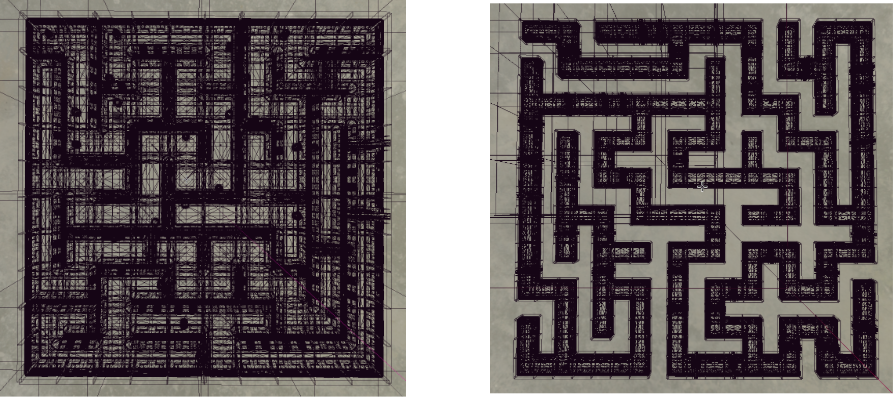
\includegraphics[width=0.8\textwidth]{diagrams/spacing.png}
    \caption{Comparison of a 10x10 maze: left without spacing, right with spacing, viewed from the top in debug mode. Notice the extra spacing making sure that parallel hallways do not touch.}
    \label{fig:maze-spacing}
\end{figure}

\subsubsection{Pathfinding}
The implementation features an efficient A* pathfinding algorithm that calculates optimal routes between any two points in the maze. This algorithm employs a Manhattan distance heuristic—particularly suitable for grid-based movement—and accounts for walls when evaluating potential paths. The pathfinding system serves dual purposes: it generates navigation routes for potential enemy AI and provides visual guidance for players through path markers that highlight the shortest route to objectives. The algorithm maintains separate data structures for tracking both the cost of the path so far (g-score) and the estimated total cost to the destination (f-score), ensuring optimal path discovery even in complex maze configurations.

\subsubsection{Random Cell Selection}
A utility function is provided to select random cells with specific properties (e.g., cells with at least one open side). This function is specifically used to choose the start and destination points within the maze, ensuring that these critical locations are appropriately positioned in accessible areas of the maze.

\subsection{Benchmark}


\section{3D World Organization}
TODO

\section{User Controls and Movement}
TODO

\section{Shortest Path Finding}
TODO

\section{Lighting and Materials}
TODO

\section{Texture Mapping}
TODO

\section{Space Partitioning: Octree}
TODO

\section{Collision Detection}
TODO

\section{Ray Intersection}
TODO

\section{Comparison with Other Space Partitioning Algorithms}
TODO

\section{Implementation Challenges}
TODO

\section{Evaluation and Results}
TODO

\section{Conclusion}
TODO

\pagebreak
\nocite{*}
\bibliographystyle{apacite}
\bibliography{references}

\end{document}
